%
\begin{figure}
%\vspace{0.2 in}
%\setlength{\epsfxsize}{10cm}%7
%\centerline{\epsfbox{ipc1.eps}}
\centering
\epsfig{file=ipc1.eps,width=5.8in}
\caption{{\em IPC Results using Singlepath Execution.} 
IPC results for several machine configurations is shown for each of
the five benchmark programs evaluated when no multipath execution
is employed.}
\label{fig:ipc1}
\end{figure}
%
\begin{figure}
%\vspace{0.2 in}
%\setlength{\epsfxsize}{10cm}%7
%\centerline{\epsfbox{ipc2.eps}}
\centering
\epsfig{file=ipc2.eps,width=5.8in}
\caption{{\em IPC Results using Simple Multipath Execution.} 
IPC results for several machine configurations is shown for each of
the five benchmark programs evaluated when the enhanced release version of
multipath execution is employed.}
\label{fig:ipc2}
\end{figure}
%
\begin{figure}
%\vspace{0.2 in}
%\setlength{\epsfxsize}{10cm}%7
%\centerline{\epsfbox{ipc3.eps}}
\centering
\epsfig{file=ipc3.eps,width=5.8in}
\caption{{\em IPC Results using the Release method of Multipath Execution.} 
IPC results for several machine configurations is shown for each of
the five benchmark programs evaluated when the enhanced release version of
multipath execution is employed.}
\label{fig:ipc3}
\end{figure}
